\chapter{Background}

This chapter will present the relevant background for this report. 

\section{Simultaneous localization and mapping}

Simultaneous localization and mapping (SLAM) is a procedure of acquiring a map of an unknown environment as a mobile platform explores it and, at the same time, localizes the mobile platform on the same map, and it is one of the key enabling technologies of mobile robot navigation \cite{Stachniss2016SimultaneousMapping}. More technically, SLAM is the procedure of estimating the sequence of robot poses, or the robot path, $X_t = \{x_0, x_1, x_2,...,x_t\}$, where $t$ denotes the time. The robot uses different sensors and/or motion models to obtain its odometry, $U_t = \{u_0, u_1, u_2,...,u_t\}$, describing the relative motion between time $t-1$ and $t$. Further, the robot uses sensors to sense the environment. The environment can be either modeled by volumetric or feature-based models. The volumetric model has a high enough resolution that allows for photo-realistic reconstruction and is a high-dimensional problem. Feature-based or landmark-based models are of a lower dimension and tend to be faster. Since this report tests landmark detectors, only feature-based SLAM is treated further. Let the pose of landmark $n$ be denoted $l_n$. Then, the robot measures the relative position between its pose, $x_t$, and the landmark poses of the landmarks in map $m$. Let the vector containing all landmark measurements at time $t$ be denoted $z_t$. The measurement of landmarks is then given by $Z_t = \{z_0, z_1, z_2,...,z_t\}$.

Factor graphs are the de-facto standard for modeling SLAM. The nodes in the graph represent the robot poses and the landmark positions, and the factors represent the odometry and landmark measurements. \cref{fig:factor_graph} shows a simple SLAM problem with four poses, $x_t$, and two landmarks, $l_n$. The odometry, $u_t$, between the poses and landmark measurements, $z_{t,n}$ of landmark $n$ at time $t$ is given as

\begin{equation}
    u_t = p(x_t \,|\, x_{t-1},u_t),
    \label{eq:odom_pdf}
\end{equation}

and

\begin{equation}
    z_{t,n} = p(z_{t,n} \,|\, x_{t-1},m).
    \label{eq:landmark_measurement_pdf}
\end{equation}

Using the factor graph formulation, the SLAM problem can be formulated as a maximum a posteriori (MAP) estimation, where the goal is to estimate the path, $X_t$, and map, $m$, that maximizes the likelihood given by

\begin{equation}
    X_t^*, m^* = \argmax_{X_t,m} \, logp(X_t,m \,|\, Z_t,U_t),
    \label{eq:SLAM}
\end{equation}

which is also often called the back-end of SLAM.

The front-end of SLAM consists of landmark extraction and data association. Landmark extraction is the procedure of finding and extracting landmarks from the sensors sensing the environment, for example, an RGB-D camera.  Data association is the procedure of determining the landmark identity of the extracted landmarks.

\begin{figure} [t]
    \centering
    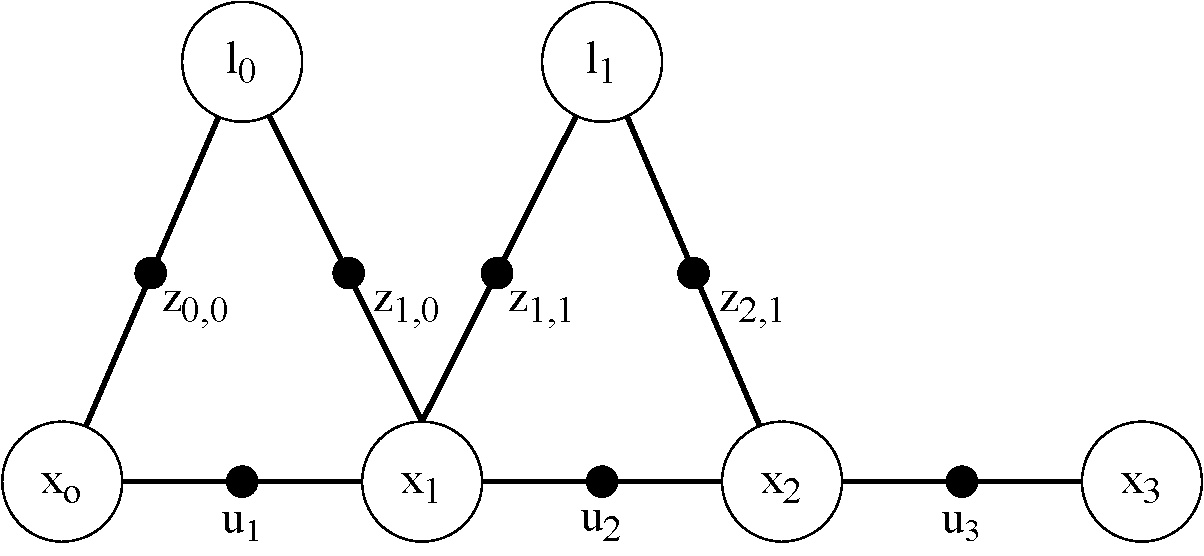
\includegraphics[width=0.6\textwidth]{figures/factor_graph.drawio.pdf}
    \caption{Factor graph of a simple SLAM problem containing four poses and two landmarks}
    \label{fig:factor_graph}
\end{figure}


Underwater SLAM is a challenging research topic, and task for underwater vehicles in long-term operation due to the limitations of subsea localization sensors and perception sensors for mapping \cite{Hidalgo2015ReviewTechniques}. The perception sensors available underwater are sonars and cameras. Sonars typically provide noisy and distorted images or low-resolution ranging, and cameras provide highly detailed images but are limited by the range of sight due to turbidity and the lack of light. For unstructured applications, often referred to as seafloor applications, side scan sonar (SSS), forward-looking sonar (FLS), and camera are the preferred perception sensors. Due to the problems with reduced range of sight for cameras and the high cost of FLS, this report focuses on landmark detection using SSS.

\section{Side scan sonar}

The side scan sonar is a two-transducer sonar where each transducer is mounted such that it points downwards and outwards to the port and starboard side of the AUV, respectively \cite{Burguera2016High-ResolutionSonar}. Each transducer transmits an ultrasonic pulse periodically and measures the echo scattered back to the transducer from the seafloor. \cref{fig:sss} shows a typical SSS setup. Each transducer is mounted with an angle, $\theta$, from the AUVs y-axis and has a sensor opening, $\alpha$, restricting the direction of the ultrasonic pulse. The echo return is measured at fixed time intervals, where each measurement is referred to as a \textit{bin}. Each of the bins corresponds to a slant range, $r_s$, proportional to the pulse's time of flight (TOF) and a gracing angle, $\theta_s$. The time between the measurement of two subsequent bins governs the slant resolution, $\delta_s$. Further, the time between two pulses governs the sensor range $r_{s, max}$. All bins between two pulses are referred to as a \textit{swath}. To form a sonar image, subsequent swaths are stacked together, as shown in \cref{fig:stacking_of_sonar_image}. 

Projecting the SSS swath to the seafloor is hard \cite{Coiras2007MultiresolutionImages}, and since the topology of the seafloor is unknown, a common assumption is to assume that the seafloor and all objects on it are flat \cite{Burguera2016High-ResolutionSonar, Shin2015BundleMapping, Burguera2014IntensityImages, Fallon2011EfficientSonar}. The flat floor assumption is used when calculating the ground range, $r_g$. The ground range represents the slant range, $r_s$, projected into the horizontal plane and is given by

\begin{equation}
    r_g = \sqrt{r_s^2 - h^2},
    \label{eq:ground_range}
\end{equation}

where $h$ is the altitude of the AUV above the seafloor.

\begin{figure}[ht]
    \centering
    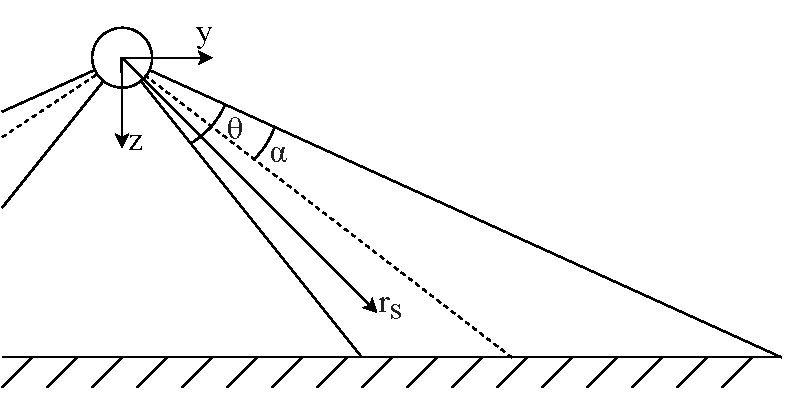
\includegraphics[trim=0cm 0cm 0cm 3.1cm, clip=true, width=0.7\textwidth]{figures/sss.drawio.pdf}
    \caption{Typical configuration of the side scan sonar.}
    \label{fig:sss}
\end{figure}

\begin{figure}[ht]
    \centering
    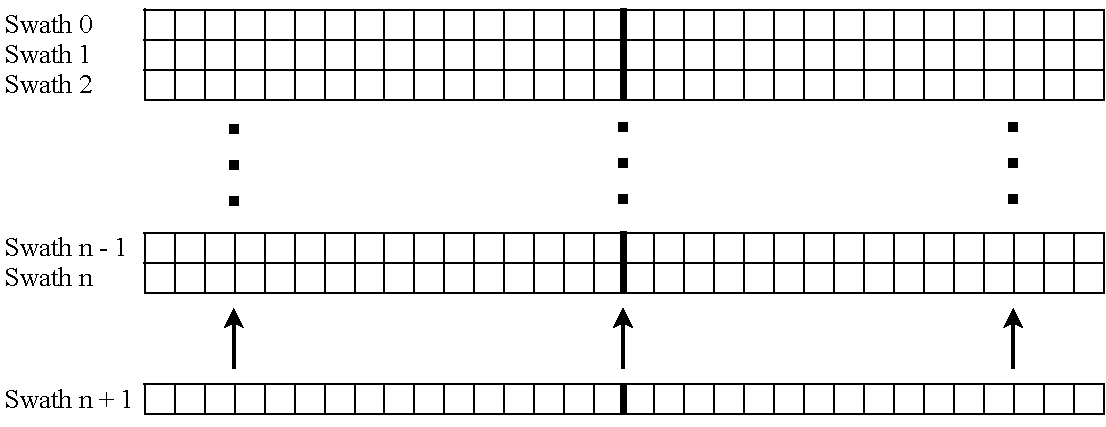
\includegraphics[width=0.7\textwidth]{figures/stacking_of_sonar_image.drawio.pdf}
    \caption{The figure shows how swaths are stacked together to form a sonar image.}
    \label{fig:stacking_of_sonar_image}
\end{figure}

\section{Data normalization and smoothing}

Cubic splines can be used to both normalize SSS data \cite{ReitanHogstad2022Side-ScanAutonomy} and to smooth the data to remove noise \cite{Al-Rawi2017LandmarkImages}. To normalize the SSS data, cubic spline regression estimates the underlying distribution of intensity values. For smoothing the SSS data, the cubic spline regression is used as the new smoothed data. The cubic smoothing spline, $f$, is 

\begin{equation}
    {f}(x) = \min_{f} p \sum_{i=1}^n |y_i-f(x_i)|^2 + (1-p) \int|D^2f(t)|^2dt,
    \label{eq:cubic_spline}
\end{equation}

where the first term is the error term and the second is the roughness measure,  where the integral is taken over the smallest interval containing all the entries of $x$. Further, $n$ is the number of data entries, $y_i$ sample $i$ of the data, $D^2f$ is the second derivate of $f$, and $p \in [0,1]$ is the smoothing parameter used to weigh between the error term and the roughness measure. 

For smoothing SSS data, each of the swaths is divided into a left and right swath, coming from the left and right transducer. Each of the parts of the swath is smoothed individually to form a cubic spline regression of the data, resulting in $\hat{I}(z) = f(z)$ for each bin, where $f$ is the smoothing cubic spline of the swath, found from \cref{eq:cubic_spline}.

Normalization, on the other hand, estimates the underlying distribution by cubic spline regression to normalize the data by

\begin{equation}
    \hat{I}(z) = \frac{I(z)}{f(z)},
    \label{eq:swath_norm}
\end{equation}

where $I(z)$ is the echo intensity at bin $z$, and again $f$ is the smoothing cubic spline of the swath, found from \cref{eq:cubic_spline}.

\section{Landmark detection}

Landmark detection is to detect interesting features, or in other words, landmarks, from data generated from observing the surroundings. For underwater applications, this can be translated to detect natural or artificial objects on the seafloor for SSS data. Due to SLAM for underwater vehicles being a challenging research topic \cite{Hidalgo2015ReviewTechniques}, the current research on landmark detection is not rich. A closely related research topic is the detection of mines on the seafloor, where the object also is to extract objects of interest on the seafloor \cite{Picard2016DetectionDimensionality}. In general, there are two main categories for detecting landmarks on the seafloor, either by classical methods, finding the echoes and/or shadows of the landmarks, or by using machine learning to extract the features. In recent years, using the rapidly evolving field of deep learning to do feature detection in sonar images has grown in popularity \cite{Wang2020ImageSonar, Zhou2022NonlinearFeatures}. However, the results generated from machine learning can be hard to explain and demands a lot of annotated data. Because of this, this report has chosen to focus on landmark detection using classical methods, and, therefore, machine learning for landmark detection will not be treated further.

Classical landmark detection methods for side scan sonar data exploit signal and image processing methods to find echoes and shadows in SSS data to extract landmarks. Classical methods can further be split into finding shadows and/or echoes in 1-dimensional swaths or 2-dimensional sonar images.

By doing peak detection, finding echoes and shadows in swaths is done in \cite{Al-Rawi2017LandmarkImages}. First, a smoothing by use of cubic splines is performed. Next, echoes are found by simple peak detection, whereas shadows are found by inverting the signal and performing peak detection. The first peak for shadows and echoes is removed since it represents the blind zone and the first bottom return (FBR), respectively, and not a landmark. A threshold based on the width and prominence of the peaks is used to remove insignificant peaks and find the landmarks.  

Landmark detection on 2D sonar images is the most common approach when doing classical landmark detection \cite{Wang2017UnderwaterSonar, Siantidis2016SideVehicles, Yuan2016AnNavigation, Leblond2019SonarProject}. The general approach uses a threshold to segment the image, either chosen arbitrarily or found adaptively. Depending on the method, the image is segmented into background, shadows, and/or echoes. Further, the shadows and/or echo landmarks are filtered to find landmarks with specific properties. \cite{Leblond2019SonarProject} filters shadows based on their geometrical properties to find consistent landmarks. 

\section{Generating consistent landmarks}

Morphological operators can be utilized to ensure consistent landmarks \cite{Yuan2016AnNavigation}. Morphological operators are a well-known image-processing tool based on a structuring element that is slid over the image, one pixel at a time, to compute new pixel values \cite{Gonzalez2018DigitalProcessing}. \cref{fig:image_processing_basics} shows the three first steps of such a process. Here the structuring element is of size $3\times3$ with the origin at the center. To ensure that the resulting image has the same size as the original image, padding can be added around the image's border. The values in the padding pixels can be chosen depending on the application. For example, it can reflect the image, replicate its border or be a constant pixel value.  

\begin{figure}
    \centering
    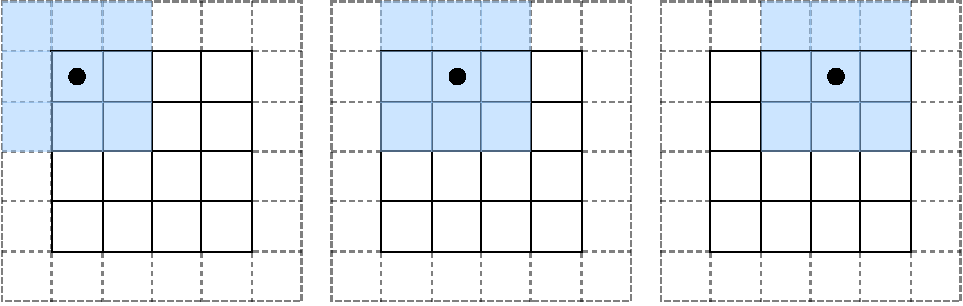
\includegraphics[width=0.8\textwidth]{figures/Image_processing_essentials.drawio.pdf}
    \caption{The image shows the three first steps (from left to right) of a general image processing method using a structuring element that is moved along the image with a stride of one to compute new pixel values. The black dot corresponds to the origin of the structuring element. The image is padded to get a new image of the same size as the old one.}
    \label{fig:image_processing_basics}
\end{figure}

The four basic morphological operators are erosion, dilation, closing, and opening, where the two latter are a combination of the first operations. As the image, the structuring element does also have binary values. If we restrict the structuring element to be of odd width and height, the erosion is defined as 

\begin{equation}
    \begin{split}
        I_s(0,0) = \prod_{i = -\frac{n-1}{2}}^\frac{n-1}{2} \prod_{j = -\frac{m-1}{2}}^\frac{m-1}{2} f(i,j) \\
        f(x,y) = 
        \begin{cases}
        I_s(x,y) & S(x,y) \neq 0 \\
        1 & otherwise
        \end{cases}
    \end{split}
    \label{eq:erosion}
\end{equation}

and the dilation as

\begin{equation}
    I_s(0,0) = min(1, \sum_{i = -\frac{n-1}{2}}^\frac{n-1}{2} \sum_{j = -\frac{m-1}{2}}^\frac{m-1}{2} I_s(i,j) \; S(i,j)).
    \label{eq:dialation}
\end{equation}

The effect of an erosion operation is that all objects are shrunk, and small objects are removed. On the other hand, dilation results in all objects being thickened and holes in objects being filled. The effects of eliminating small objects and filling holes help generate consistent landmarks. However, the side effect of shrinking and thickening objects are unwanted. A dilation and erosion operation is combined to revert the side effects, and the new operations are called opening and closing. An opening operation is an erosion followed by a dilation, effectively removing small objects from the image. Closing is a dilation followed by erosion, eliminating holes in the image. 
